\section{Extensions}
\label{sec:extend}

In this section, we consider the generalization to the unambiguous discrimination scheme, non-uniform prior probabilities, and quantum noise.

\subsection{Unambiguous Discrimination Measurement}
\label{subsec:ud}

Till now, we have only considered the minimum error measurement scheme wherein the measurement operator always outputs a state, 
though sometimes incorrectly and thus incurring a certain probability of error. 
We now consider an alternative measurement scheme of unambiguous measurement~\cite{Barnett-review} where there are no errors, 
but the measurement can fail, i.e. giving an inconclusive outcome.
The unambiguous measurement scheme thus may incur a probability of failure. 
%%%%%
Fortunately, our results for the minimum error measurement scheme also hold for the unambiguous discrimination measurement scheme and objective, as observed below.

\begin{enumerate}
\item
The sufficient and necessary condition for orthogonality derived in Theorem~\ref{thm:nsensors} is a property of the states and the operator $U$, 
and is independent of the measurement scheme. Thus, Theorem~\ref{thm:nsensors}
hold for an unambiguous discrimination scheme.

\item
The intuition behind Conjecture~\ref{conj:opt} is  based on the homogeneity of
sensors and symmetry of the problem setting (e.g., symmetric eigenvalues of 
$U$, uniform probability of final states, etc.). Thus, we believe the optimal
initial state solution for an unambiguous discrimination scheme is the same as in
the case of the minimum error scheme. Thus, Conjecture~\ref{conj:opt} should hold.

\item 
Conjecture~\ref{conj:avg} is independent of the measurement scheme.

\item 
We prove the version of Lemma~\ref{lemma:angle} corresponding to the unambiguous measurement below. Thus, Theorem~\ref{thm:final} also holds for unambiguous measurement. 

\item 
The optimization problem of determining the optimal measurement $\{\Pi_i\}$ for 
an unambiguous discrimination scheme can also be formulated as an SDP~\cite{Bae_2015}, 
and thus can be computed numerically. Thus, the search heuristics from \S\ref{sec:searching} will also work for unambiguous measurement with the 
corresponding SDP for an unambiguous discrimination scheme.

% \item 
% We make the same empirical observations in our simulations for the unambiguous discrimination scheme. See below.
\end{enumerate}

\begin{lem-prf}
Consider $n$ states to be discriminated $\phi_0, \phi_1, \ldots, \phi_{n-1}$ 
such that $\bra{\phi_i}\ket{\phi_j} = x$,
for all $0 \leq i, j \leq n-1$ and $i \neq j$. 
The probability of {\bf failure} in discriminating 
$\phi_0, \phi_1, \ldots, \phi_{n-1}$ using an optimal measurement (for unambiguous
discrimination) 
increases with an increase in $x$ when $x \geq 0$.
\label{lemma:unambiguous}
\end{lem-prf}
\begin{prf}
The optimal/minimum probability of failure using the optimal POVM for a set of states with equal pairwise inner products is equal to $x$ when $x \geq 0$~\cite{quantum_pyramid}.
Thus, the lemma trivially holds. 
\end{prf}


\subsection{Non-uniform Prior Probability}
Till now, we have implicitly assumed that the events (of affecting one sensor) occur with
a uniform probability. Here, we consider the generalization of allowing for the events to occur
with non-uniform probability. This could happen if different sensor locations can have different
probabilities of the event occurrence.


\para{Number of Sensors $n=2$}. 
When the number of sensors is 2, we observe that the optimal solution for the \iso problem actually remains unchanged. 
In particular, the expression for the minimum probability of error in discriminating the two final states, with
non-uniform probabilities $p_1$ and $p_2$, for a given initial state $|\psi\rangle$ is given by (derived from~\cite{helstrom}):  
\begin{equation}
P_{e} = \frac{1}{2} \left( 1 - \sqrt{ 1 - 4 p_1 p_2 |\langle \psi |(U\otimes U^{-1} ) |\psi\rangle |^{2}} \right). 
\label{eqn:two-prior}
\end{equation}
The above entails that, as for the case of uniform probabilities, we need to minimize $ |\langle \psi |(U\otimes U^{-1} ) |\psi\rangle |$,
 which is independent of $p_1$ and $p_2$. Thus, the optimal initial state for $n=2$ is independent of the probabilities associated with the final states/events.

\para{Number of Sensors $n > 2$.} 
For $n>2$, it is easy to see that Theorems~\ref{thm:3sensor} and~\ref{thm:nsensors} that derive
conditions for orthogonality of the final states remain unchanged since the probabilities of 
events/final-states do not affect the final states themselves. 
%%%%%%%%%%
However, the optimal \iso solution for general values of $\theta$ is certainly different
than that conjectured in Conjecture~\ref{conj:opt}, since Conjecture~\ref{conj:opt} is fundamentally
based on the symmetry of the final states, which is unlikely to be the case for non-uniform probabilities of
events.
%%%%%
On the other hand, it is easy to generalize the search heuristics for the case of non-uniform probability. See Fig.~\ref{fig:non-uniform-heuristics}, which plots the objective value $P()$ 
for varying $\theta$ for the three search heuristics. We observe that (i) The heuristics return
an optimal objective value (of zero) for the conditions in Theorems~\ref{thm:nsensors}; (ii) All the heuristics perform almost the same. 
These observations suggest that the heuristics likely perform near-optimally even for the 
general case of non-uniform event probabilities.
In addition, we note that, compared to the uniform probability case 
(i.e., Fig.~\ref{fig:heuristics}), the optimal objective value $P()$ 
under non-uniform probabilities is lower than the $P()$ under uniform probabilities, 
for any particular $\theta$.

\begin{figure}[ht]
    \centering
    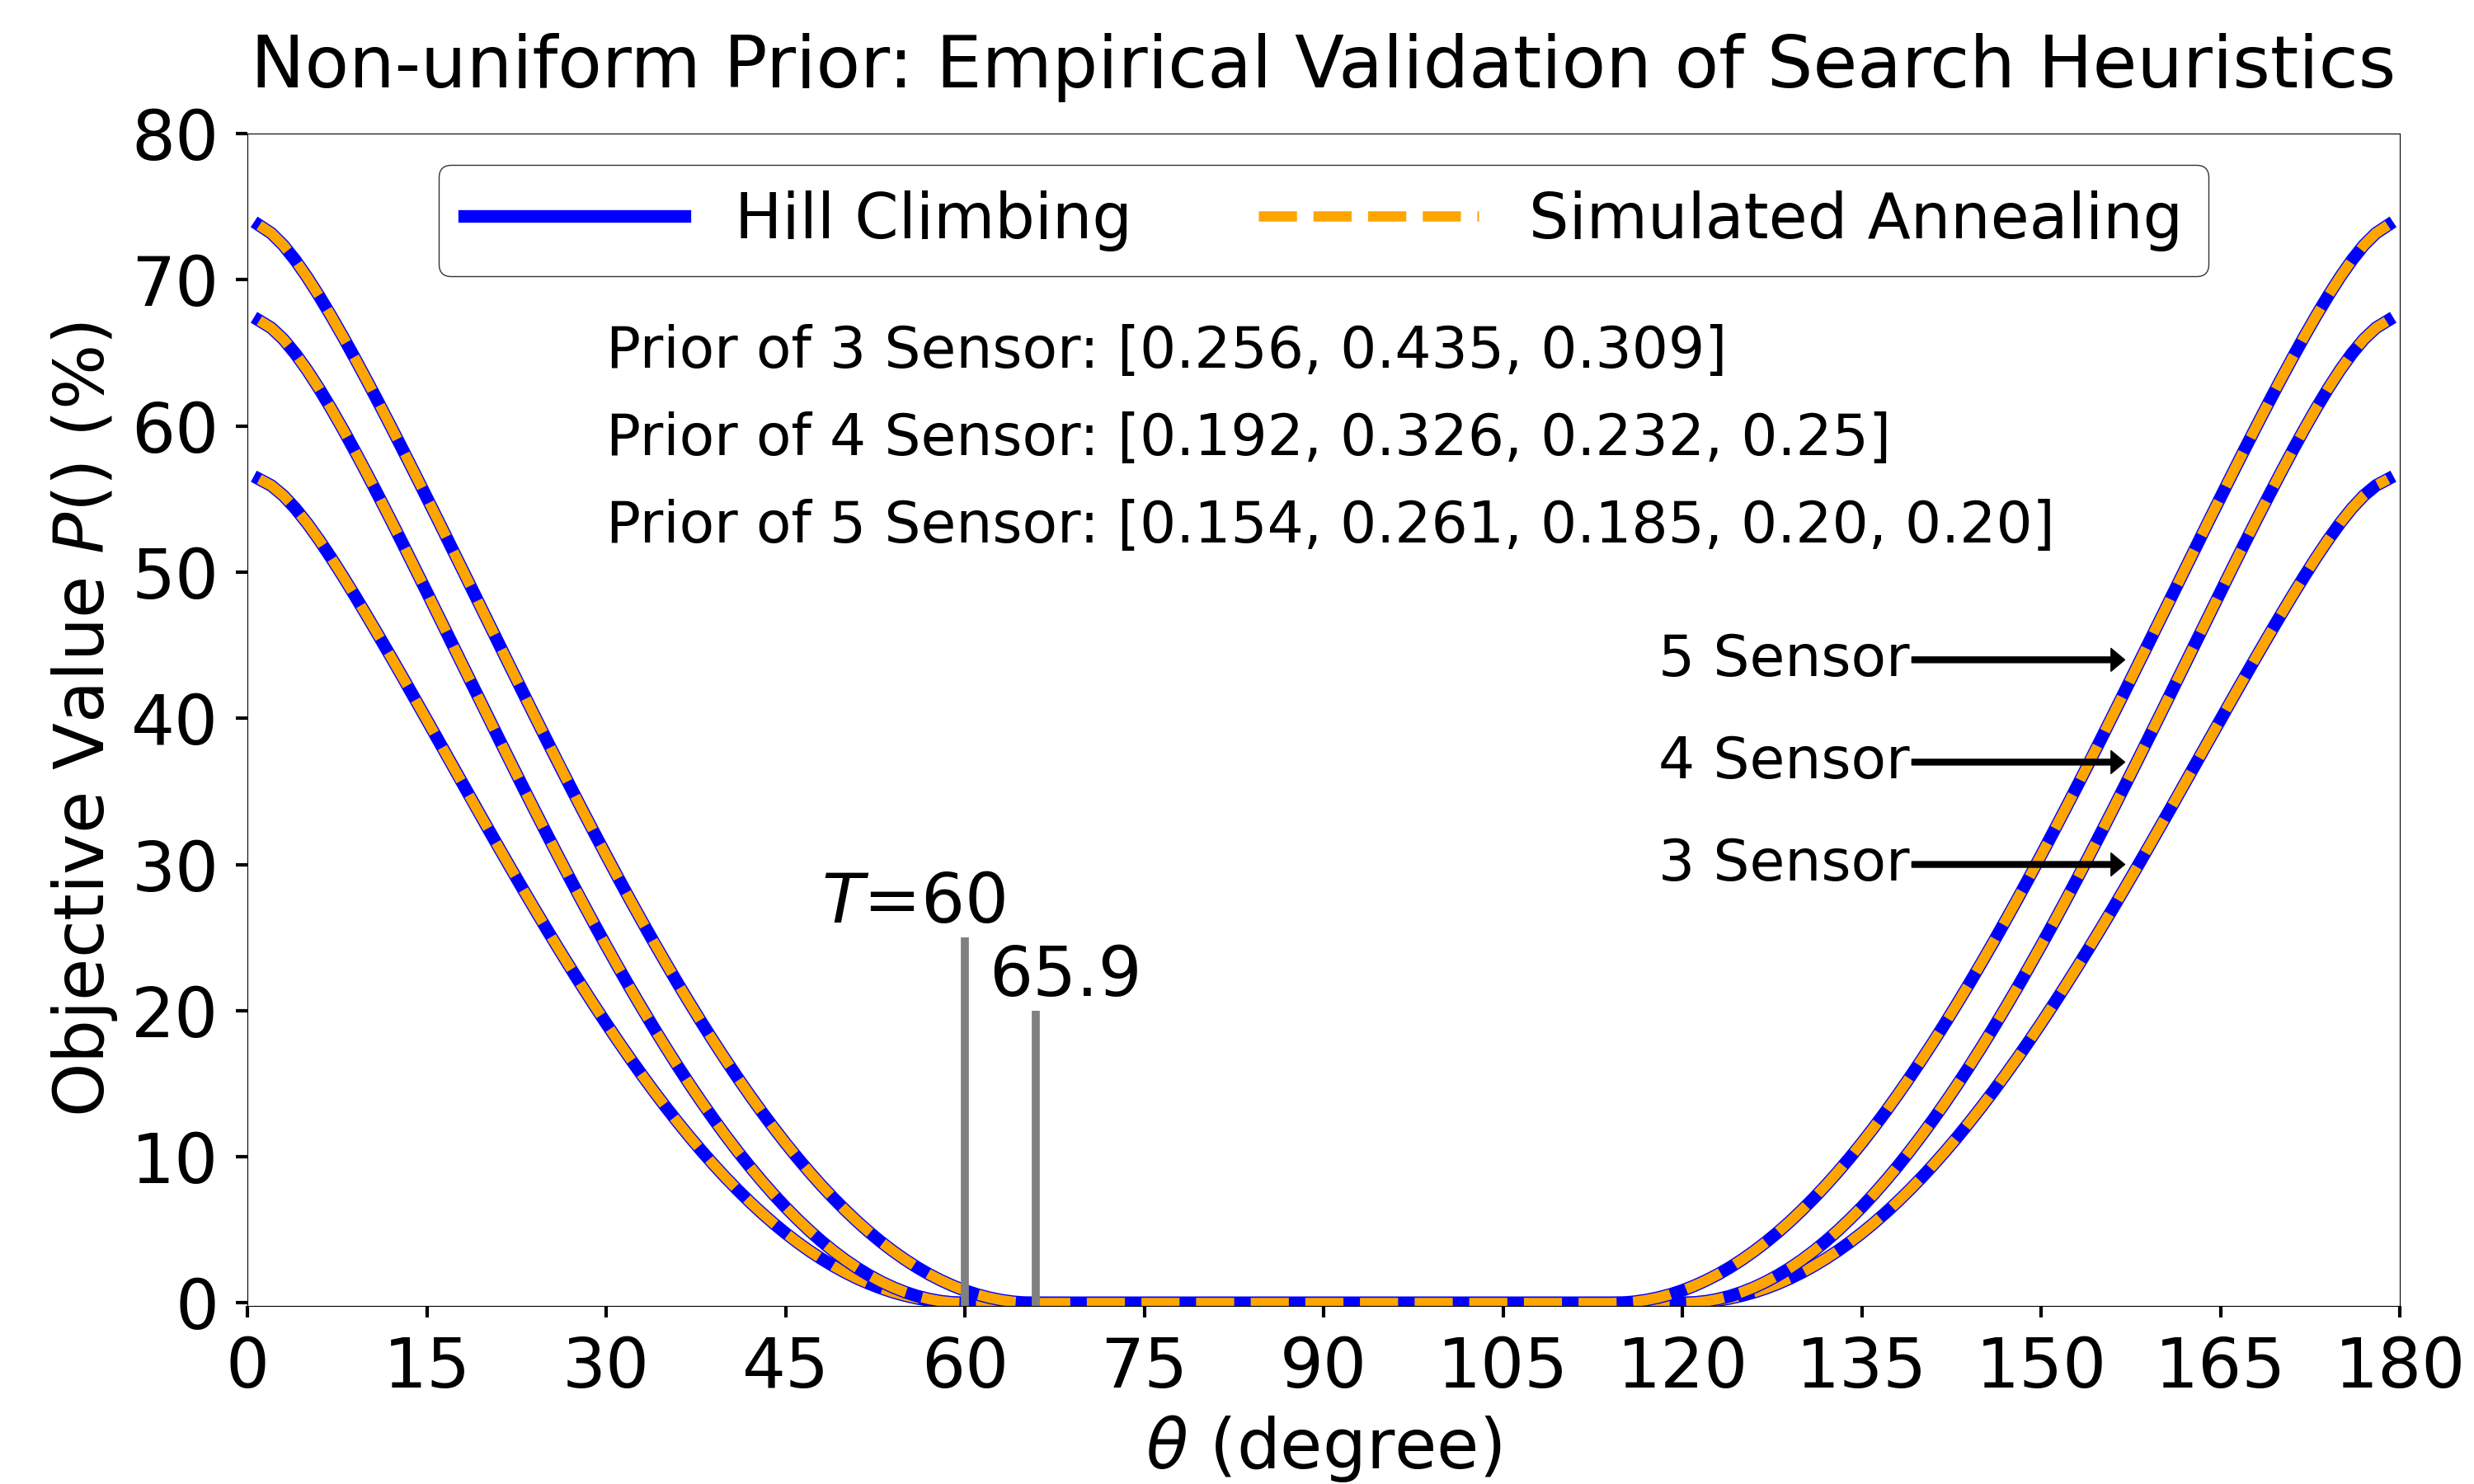
\includegraphics[width=0.8\textwidth]{chapters/tqc/figures/varying_theta_nonequal_prior.png}
    \caption{Performance of the three search heuristics with non-uniform prior for varying $U$'s parameter $\theta$, 
             for a different number of sensors in the network. Genetic Algorithm (GA) is not shown explicitly, for clarity, 
             but it also performs almost the same as Hill-Climbing and Simulated Annealing (SA), which are plotted above.}
    \label{fig:non-uniform-heuristics}
\end{figure}

\subsection{Impact of Quantum Noise.}
\label{subsec:affect_noise}
Till now, we have looked at the \iso problem from a theoretical perspective while ignoring the quantum noise. 
Since quantum noise is an essential aspect of quantum systems, we present a mitigation strategy to correct for quantum noise and evaluate it for two quantum noise models.


\para{Quantum Noise-Mitigation Strategy.}
In our context, the impact of the noise is that it essentially results in final states that are different (due to noise) than the ones we try to discriminate. 
That is, 
consider an given initial state $\ket{\psi}$ which yields (noiseless) final states $\{ \ket{\phi_i}\}$; let the optimal measurement to discriminate the final states $\{ \ket{\phi_i}\}$ be the POVM with elements $\{ E_i\}$.
%%%%%%%%%%%%%%
However, due to the noise, the actual noisy final states may actually be different than $\{ \ket{\phi_i}\}$, which, when discriminated with the POVM $\{ E_i\}$, will result
in a higher probability of error than if there were no noise.
%%%%%%%%%%%%%%%
Thus, to account for such quantum noise, we propose to modify the POVM measurement appropriately. In particular, we compute the POVM measurement to discriminate 
the expected noisy final states---which we represent by the density matrices of the 
mixed states representing the ensemble of potential final states. 
More formally, our strategy is as follows: For each final state $\ket{\phi_i}$, let $\rho_i$ be the density matrix that represents the distribution/mixture of noisy final states that may
result instead of $\ket{\phi_i}$. 
Then, we use SDP (Eqn.~\ref{eqn:measure-sdp}) to determine the optimal POVM $\{ E'_i\}$ that optimally discriminates the density matrices $\{\rho_i\}$, 
and use it to discriminate the noisy final state.

\begin{figure}[b]
    \centering
    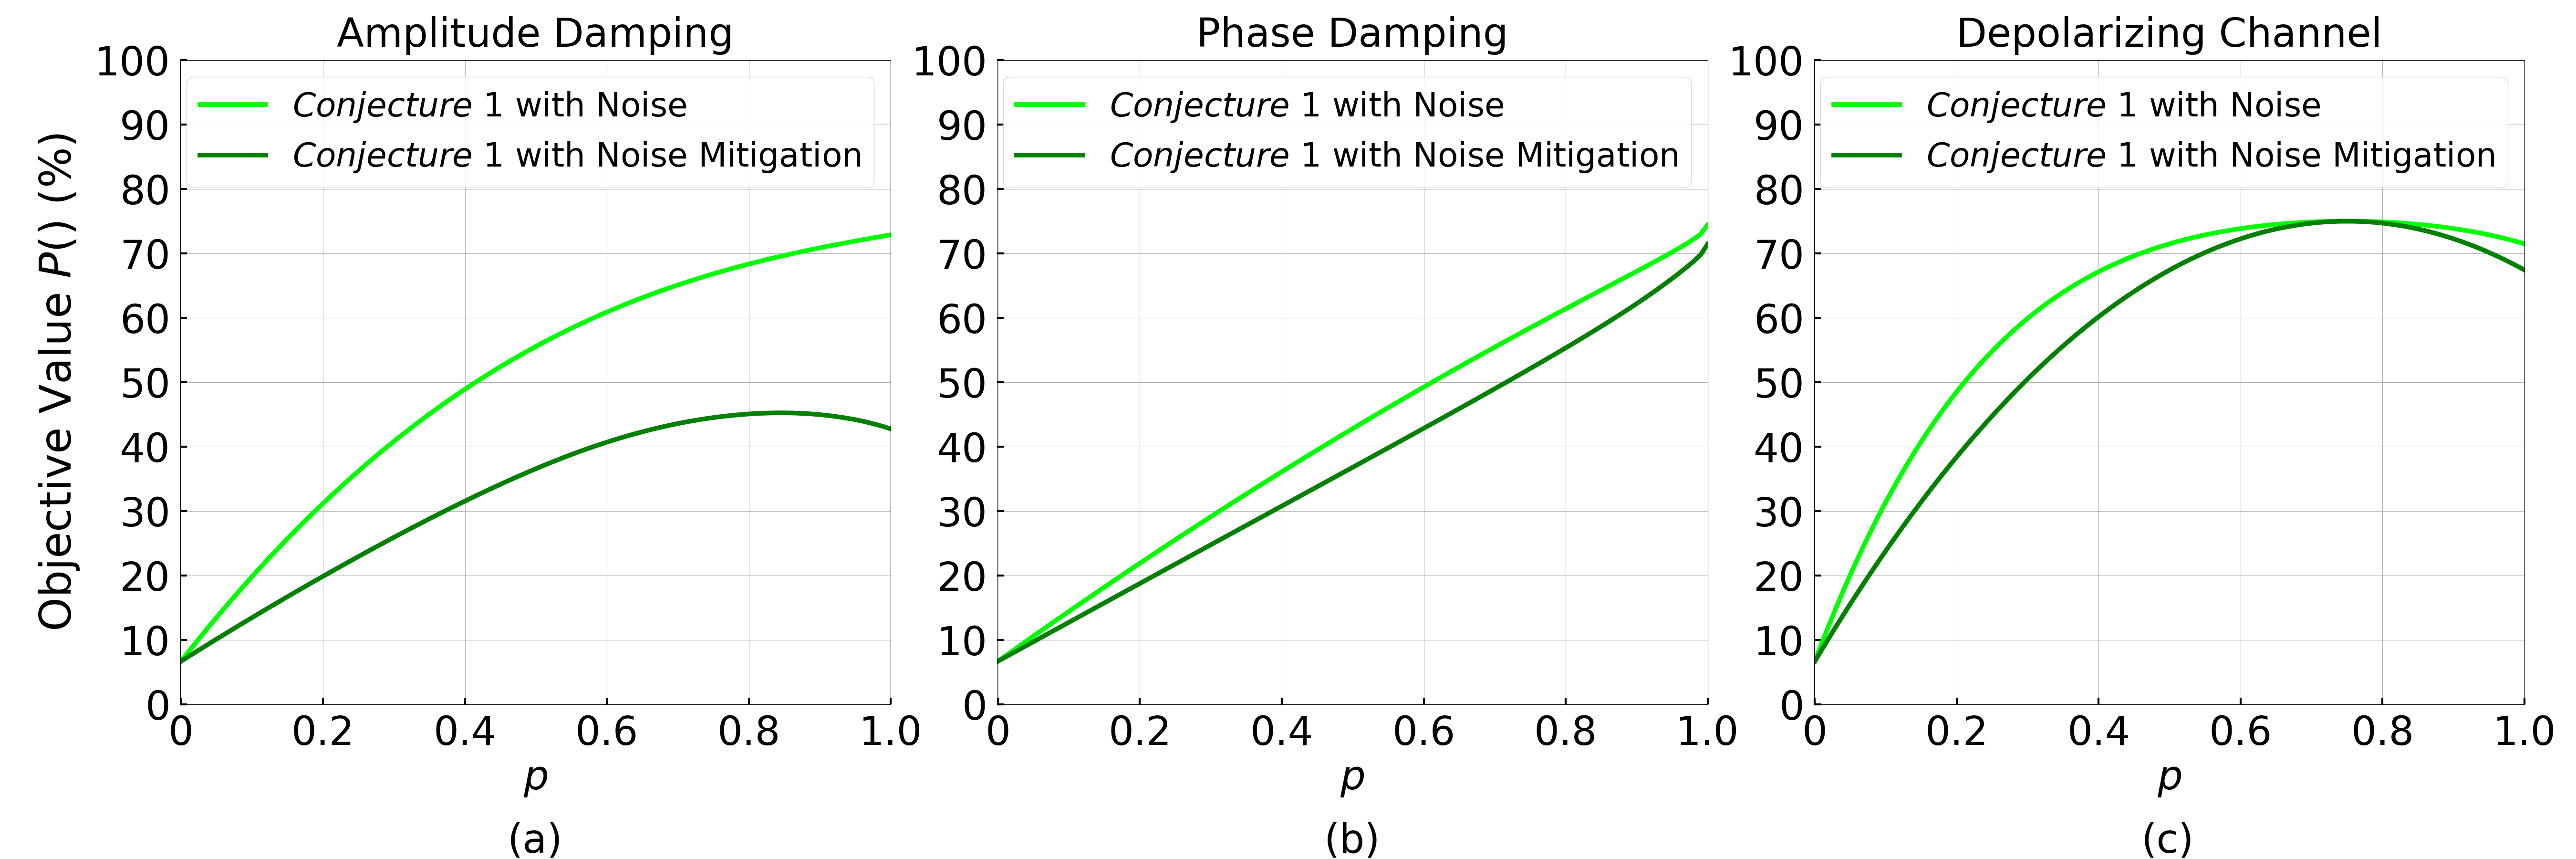
\includegraphics[width=0.99\textwidth]{chapters/tqc/figures/povmnoise.png}
    \caption{The improvement in the objective value $P()$ for the Conjecture~1's solution due to the noise-mitigation strategy, for the three noise models, for $\theta=45$ degrees and four sensors.}
    \label{fig:povm_noise}
\end{figure}


\para{Evaluation.}
We consider three popular noise models~\cite{nielsen2010quantum} for evaluation of our above mitigation technique. 
\begin{enumerate}
    \item \emph{Amplitude damping} causes the quantum system to lose energy.
    \item \emph{Phase damping} describes the loss of quantum information without energy loss.
    \item \emph{Depolarizing channel} is probabilistically replacing the qubit by the completely mixed state, $I/2$.
\end{enumerate}
All the above noise models can be characterized using the Kraus operators ($K$), which obey $\sum_{i} K_{i}^{\dagger}K_i=I$. In particular, the Kraus operators for the amplitude damping are:
$$ \mathcal{N}_{amp} = \{K_{a0}, K_{a1}\} = \{ \begin{bmatrix}
  1 & 0 \\
  0 & \sqrt{1 - p} \\
\end{bmatrix}, 
\begin{bmatrix}
  0 & \sqrt{p} \\
  0 & 0 \\
\end{bmatrix} \}$$
where $p$ can be thought of as the probability of losing a photon~\cite{nielsen2010quantum}. 
% In the above, the noise due to Kraus operator $K_{a0}$ occurs with a probability of $(1-p)$ and due to $K_{a1}$ with a probability of $p$.
The Kraus operators for the phase damping are:
$$ \mathcal{N}_{pha} =   \{K_{p0}, K_{p1}\} = \{ \begin{bmatrix}
  1 & 0 \\
  0 & \sqrt{1 - p} \\
\end{bmatrix}, 
\begin{bmatrix}
  0 & 0 \\
  0 & \sqrt{p} \\
\end{bmatrix} \}$$
where $p$ can be interpreted as the probability that a photon from the system has been scattered (without loss of energy)~\cite{nielsen2010quantum}.
Finally, the Kraus operators for the depolarizing channel are:
% \{\sqrt{1-p}I, \sqrt{\frac{p}{3}}X, \sqrt{\frac{p}{3}}Y, \sqrt{\frac{p}{3}}Z\} =
$$ \mathcal{N}_{dep} = \{K_{d0}, K_{d1}, K_{d2}, K_{d3}\} =  \{\sqrt{1-p}\begin{bmatrix}
  1 & 0 \\
  0 & 1 \\
\end{bmatrix}, \sqrt{\frac{p}{3}}\begin{bmatrix}
  0 & 1 \\
  1 & 0 \\
\end{bmatrix}, \sqrt{\frac{p}{3}}\begin{bmatrix}
  0 & -i \\
  i & 0 \\
\end{bmatrix}, \sqrt{\frac{p}{3}}\begin{bmatrix}
  1 & 0 \\
  0 & -1 \\
\end{bmatrix} \}$$
where $p$ is the probability of a qubit being depolarized.
%%%%%%%%%%%%%%%%%%%%%%%%%%%%%%%%%%%
For a given noise model, its Kraus operators give the operators by which the state's density matrix is transformed with a corresponding probability. 
%%%%%%%%%%%%%%%
For example, in our context, under the third noise model of depolarizing noise, for a given initial state $\ket{\psi}$, 
each final state $\ket{\phi_i}$ with a density matrix $\rho_i = \ketbra{\phi_i}$ is transformed to $K_{d0}\rho_i K^{\dagger}_{d0}$ with a probability of $(1-p)$ and to $K_{d1}\rho_i K^{\dagger}_{d1}$ or $K_{d2}\rho_i K^{\dagger}_{d2}$ or 
$K_{d3}\rho_i K^{\dagger}_{d3}$ with a 
probability of $p/3$ each.
%%%%%%%%%%%%%%%%%%%%%%%%%%%%%%%%%%%%%%%%%%%%%%%%%
%%%%%%%%%%%%%%%%%%%%%%%%%%
The above noise models are for a single sensor/qubit; 
for multiple qubits, we use a tensor product of the single-qubit noises.
% Now, for an initial state $\rho = \ketbra{\psi}$, the noisy final states $\{\rho_i\} = \{  
% \mathcal{V}_{i}({\mathcal{N}(\rho)}) \}$, where $\mathcal{N} \in \{  \mathcal{N}_{amp}, \mathcal{N}_{pha}, \mathcal{N}_{dep} \}$, $\mathcal{V}_i = I^{\otimes i} \otimes U \otimes I^{\otimes (n-i-1)}$, and $U$ is defined in \S\ref{sec:problem}.
Fig.~\ref{fig:povm_noise} shows the 1) impact of various quantum noise on the results, and 2) for the initial state (from Conjecture~1),
how the objective value $P()$ improves due to the above-discussed noise-mitigation strategy for the three noise models, for the specific value of $\theta = 45$ degrees and the number of sensors equal to 4.
%%%%%%%%%%%%%%%%%%%%%%
We observe that the improvement is particularly significant in the case of amplitude-damping noise.


%  larger the objective value, i.e., a higher error in discriminating the noisy final states.
% Also, the dark green lines have a smaller objective value than the shallow green lines, which shows that the account-for-noise modification has improved in decreasing the error in discriminating the noisy final states.
% In particular, the modification is more effective for amplitude damping compared with the other two types of noise.}


% The difference between amplitude damping and phase damping is in $K_1$.
% In amplitude damping, the $K_1$ changes a $\ket{1}$ state into a $\ket{0}$ state, corresponding to the physical process of losing a photon.
 % i.e., the relative phase between $\ket{0}$ and $\ket{1}$ is lost.
%%%%%%%%%%%%
% We model the coherent noise as a $Z$ rotation operator~\cite{coherentnoise}:
% $$ \{K_0\} = \{RZ(\epsilon) \}= 
% \begin{bmatrix}
%   e^{-i\frac{\epsilon}{2}} & 0 \\
%   0 & e^{i\frac{\epsilon}{2}} \\
% \end{bmatrix},
% $$
% where $\epsilon$ is the rotation angle caused by noise. 
%%%%%%%%%%%%

% So for $n$ sensors, the number of Kraus operators for our coherent noise is one ($1^n$), while the number of Kraus operators for our incoherent noise is $4^n$.
% \blue{To observe how the optimal initial state behaves under the presence of noise, we do quantum state discrimination on the noisy final states using the POVM $\{ E_i \}$ computed from noiseless final states.
% The details are as follows:
% \begin{enumerate}
%     \item Compute the POVM $\{ E_i \}$ using semi-definite programming (SDP) on the noiseless final states $\{ \ket{\phi_i} \}$ evolved from the proposed optimal initial state $\ket{\psi}$.
%     \item The quantum sensor network outputs a noisy final state $\phi_i$ from a set of noisy final states $\{ \phi_i \}$ that evolved from a noisy initial state $\psi$.
%     Here $\psi$ and $\phi$ without ket notations represent density matrices.
%     $\psi = \sum_i K_i \ketbra{\psi} K_i^{\dagger}$, $\phi_i = V_i \psi V_i^{\dagger}$, $ V_i=I^{\otimes i} \otimes U \otimes I^{\otimes (n-i-1)}$, and $U$ is defined in \S\ref{sec:problem}.
%     \item Measure a noisy final state $\phi_i$ with $\{ E_i \}$ and check whether the quantum state discrimination is correct or not.
%     \item Repeat steps (2)--(3) many times and finally compute the average probability of error.
% \end{enumerate}
% The experiment evaluation metric is the average probability of error in the quantum state discrimination (QSD) with the minimum error strategy.
% }




% In Fig.~\ref{fig:povm_noise} (a), the modification has a significant improvement, where the probability of error in the QSD increased from $4.9\%$ to $25.4\%$, which is significantly smaller than increasing to $65.8\%$ without the modification.
% In Fig.~\ref{fig:povm_noise} (b), the modification still has an improvement, but the improvement is much smaller.
% This implies that the depolarising error is more difficult to account for.




% \softpara{Account for Noise.}
% \blue{We make a simple modification to account for quantum noise.
% We do not modify our proposed optimal initial state, but instead update the way the POVM operators are computed.
% In \S~\ref{subsec:affect_noise}, the POVM is computed using noiseless final states evolved from a noiseless initial state.







% \blue{In Fig.~\ref{fig:phaseshift_noise} (a) where the input unitary's $\theta=20$, we observe that for our Conjecture~\ref{conj:opt}, the probability of error in the QSD increases as the phase shift $\epsilon$ increases\CZ{what is a reasonable value in practice?}.
% %and the error increase rate first goes up (concave up) before 60 degrees, then the error increase rate goes down (concave down) after 60 degrees.
% We also observe that the probability of error for the \texttt{Uniform-all} is always larger than the error for the proposed initial state.
% Note that the Y-axis value of the data point ($\epsilon=0, 34.3\%$), implying noiseless, is nearly the same as the 3 Sensors dashed line at data point ($\theta=20, 34.4\%$) in Fig.~\ref{fig:conjecture} where there is no noise.
% The $0.1\%$ difference comes from the fact that in Fig.~\ref{fig:conjecture}, the probability of error is the objective function value directly from the SDP solver~\cite{diamond2016cvxpy}, while in Fig.~\ref{fig:phaseshift_noise} the probability of error is an average of repeating multiple measurement results.
% Fig.~\ref{fig:phaseshift_noise} (b) has similar patterns with (a).
% But for (c) where the unitary's $\theta=70$, the difference between our Corollary~\ref{cor:orthogonal-opt} and the \texttt{uniform-all} is small.
% At phase shift $\epsilon=0$, the probability of error is zero for the Corollary~\ref{cor:orthogonal-opt}, and $0.7\%$ for the \texttt{uniform-all}.
% The probability of error for our Corollary~\ref{cor:orthogonal-opt} is slightly higher than the \texttt{uniform-all} between $20$ and $100$ degrees.
% }

% \blue{In Fig.~\ref{fig:depolar_noise} (a) where the input unitary's $\theta=20$, we observe that for our Conjecture~\ref{conj:opt}, the probability of error in the QSD increases when the probability $p$ of Pauli X, Y, Z increases.
% We also observe that our Conjecture~\ref{conj:opt} only gives an advantage against \texttt{Uniform-all} in the range of $p \in [0, 16]$ percentage.
% The pattern is similar for Fig.~\ref{fig:depolar_noise} (b) and (c) where the input unitary's $\theta$ equals $45$ and $70$ degrees respectively, except that the range wherein our optimal initial state gives an advantage against the \texttt{Uniform-all} becomes smaller.
% In Fig.~\ref{fig:depolar_noise} (b), the range is $p \in [0, 10]$ percentage. 
% In Fig.~\ref{fig:depolar_noise} (c), the range is $p \in [0, 1]$ percentage. 
% }




% \begin{figure}[t]
%     \centering
%     \includegraphics[width=\textwidth]{figures/noise_affect_phaseshift.png}
%     \caption{3 sensor setting. How our proposed optimal initial state and \texttt{Uniform-all} behave in the presence of varying coherent phase shift $\epsilon$. The input unitary's $\theta$ in (a), (b), and (c) are 20, 45, and 70 degrees respectively. \magenta{Shall the y-axis label be P()?}}
%     \label{fig:phaseshift_noise}
% \end{figure}

% \begin{figure}[t]
%     \centering
%     \includegraphics[width=\textwidth]{figures/noise_affect_depolar.png}
%     \caption{3 sensor setting. How our proposed optimal initial state, and \texttt{Uniform-all} behave in the presence of varying incoherent depolarising probability $p$. 
%     The input unitary's $\theta$ in (a), (b), and (c) are 20, 45, and 70 degrees respectively.}
%     \label{fig:depolar_noise}
% \end{figure}



% To observe how the optimal initial state behaves under the presence of noise, we do quantum state discrimination on the noisy final states using the POVM $\{ E_i \}$ computed from noiseless final states.
% The details are as follows:
% \begin{enumerate}
%     \item Compute the POVM $\{ E_i \}$ using semi-definite programming (SDP) on the noiseless final states $\{ \ket{\phi_i} \}$ evolved from the proposed optimal initial state $\ket{\psi}$.
%     \item The quantum sensor network outputs a noisy final state $\phi_i$ from a set of noisy final states $\{ \phi_i \}$ that evolved from a noisy initial state $\psi$.
%     Here $\psi$ and $\phi$ without ket notations represent density matrices.
%     $\psi = \sum_i K_i \ketbra{\psi} K_i^{\dagger}$, $\phi_i = V_i \psi V_i^{\dagger}$, $ V_i=I^{\otimes i} \otimes U \otimes I^{\otimes (n-i-1)}$, and $U$ is defined in \S\ref{sec:problem}.
%     \item Measure a noisy final state $\phi_i$ with $\{ E_i \}$ and check whether the quantum state discrimination is correct or not.
%     \item Repeat steps (2)--(3) many times and finally compute the average probability of error.
% \end{enumerate}